% 2.8 Interactive Jobs
% -------------------------------------------------------------
\subsection{Interactive Jobs}
\label{sect:interactive-jobs}

Interactive job sessions allow you to interact with the system in real-time.
These sessions are particularly useful for tasks such as testing, debugging, optimizing code,
setting up environments, and other preparatory work before submitting batch jobs.

%  2.8.1 Command Line
% -------------------
\subsubsection{Command Line}
\label{sect:command-line}

To request an interactive job session, use the \texttt{salloc} command with appropriate options.
This is similar to submitting a batch job but allows you to run shell commands interactively
within the allocated resources. For example:
\begin{verbatim}
	salloc -J interactive-test --mem=1G -p ps -n 8
\end{verbatim}

Within the allocated \tool{salloc} session, you can run shell commands as usual.
It is recommended to use \tool{srun} for compute-intensive steps within \tool{salloc}.
If you need a quick, short job just to compile something on a GPU node,
you can use an interactive srun directly. For example, a 1-hour allocation:

\textbf{For tcsh}:
\begin{verbatim}
	srun --pty -n 8 -p pg --gpus=1 --mem=1G -t 60 /encs/bin/tcsh
\end{verbatim}
\textbf{For bash}:
\begin{verbatim}
	srun --pty -n 8 -p pg --gpus=1 --mem=1G -t 60 /encs/bin/bash
\end{verbatim}

% 2.8.2 Graphical Applications
% -----------------------------
\subsubsection{Graphical Applications}
\label{sect:graphical-applications}

To run graphical UI applications (e.g., MALTLAB, Abaqus CME, IDEs like PyCharm, VSCode, Eclipse, etc.) on Speed,
you need to enable X11 forwarding from your client machine Speed then to the compute node.
To do so, follow these steps:
\begin{enumerate}
\item Run an X server on your client machine:
\begin{itemize}
    \item \textbf{Windows:} Use MobaXterm with X turned on, or Xming + PuTTY with X11 forwarding, or XOrg under Cygwin
    \item \textbf{macOS:} Use XQuarz -- use its \tool{xterm} and \texttt{ssh -X}
    \item \textbf{Linux:} Use \texttt{ssh -X speed.encs.concordia.ca}
\end{itemize}
For more details, see \href{https://www.concordia.ca/ginacody/aits/support/faq/xserver.html}{How do I remotely launch X(Graphical) applications?}

\item Verify that X11 forwarding is enabled by printing the \api{DISPLAY} variable:
\begin{verbatim}
    echo $DISPLAY
\end{verbatim}

\item Start an interactive session with X11 forwarding enabled (Use the \option{--x11} with \tool{salloc} or \tool{srun}), for example:
\begin{verbatim}
    salloc -p ps --x11=first --mem=4G -t 0-06:00
\end{verbatim}

\item Once landed on a compute node, verify \api{DISPLAY} again.

\item Set the \api{XDG\_RUNTIME\_DIR} variable to a directory in your \tool{speed-scratch} space:
\begin{verbatim}
    mkdir -p /speed-scratch/$USER/run-dir
    setenv XDG_RUNTIME_DIR /speed-scratch/$USER/run-dir
\end{verbatim}

\item Launch your graphical application:
\begin{verbatim}
    module load matlab/R2023a/default
    matlab
\end{verbatim}
\end{enumerate}

\noindent\textbf{Note:} with X11 forwarding the graphical rendering is happening on your client machine!
That is you are not using GPUs on Speed to render graphics,
instead all graphical information is forwarded from Speed to your desktop or laptop over X11,
which in turn renders it using its own graphics card. Thus, for GPU rendering jobs either keep them
non-interactive or use VirtualGL.

\noindent Here's an example of starting PyCharm (see \xf{fig:pycharm}).
\textbf{Note:} If using VSCode, it's currently only supported with the \tool{--no-sandbox} option.

\textbf{TCSH version:}
\small
\begin{verbatim}
    ssh -X speed (XQuartz xterm, PuTTY or MobaXterm have X11 forwarding too)
    [speed-submit] [/home/c/carlos] > echo $DISPLAY
    localhost:14.0
    [speed-submit] [/home/c/carlos] > cd /speed-scratch/$USER
    [speed-submit] [/speed-scratch/carlos] > echo $DISPLAY
    localhost:13.0
    [speed-submit] [/speed-scratch/carlos] > salloc -pps --x11=first --mem=4Gb -t 0-06:00
    [speed-07] [/speed-scratch/carlos] > echo $DISPLAY
    localhost:42.0
    [speed-07] [/speed-scratch/carlos] > hostname
    speed-07.encs.concordia.ca
    [speed-07] [/speed-scratch/carlos] > setenv XDG_RUNTIME_DIR /speed-scratch/$USER/run-dir
    [speed-07] [/speed-scratch/carlos] > /speed-scratch/nag-public/bin/pycharm.sh
\end{verbatim}
\normalsize

\textbf{BASH version:}
\small
    \begin{verbatim}
    bash-3.2$ ssh -X speed (XQuartz xterm, PuTTY or MobaXterm have X11 forwarding too)
    serguei@speed's password:
    [serguei@speed-submit ~] % echo $DISPLAY
    localhost:14.0
    [serguei@speed-submit ~] % salloc -p ps --x11=first --mem=4Gb -t 0-06:00
    bash-4.4$ echo $DISPLAY
    localhost:77.0
    bash-4.4$ hostname
    speed-01.encs.concordia.ca
    bash-4.4$ export XDG_RUNTIME_DIR=/speed-scratch/$USER/run-dir
    bash-4.4$ /speed-scratch/nag-public/bin/pycharm.sh
\end{verbatim}
\normalsize

\begin{figure}[htpb]
	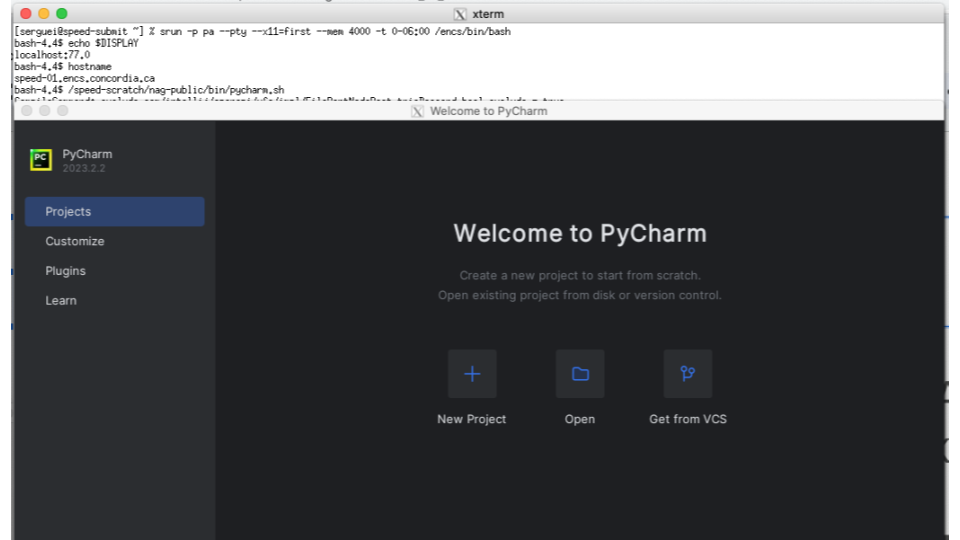
\includegraphics[width=\columnwidth]{images/pycharm}
	\caption{Launching PyCharm on a Speed Node}
	\label{fig:pycharm}
\end{figure}

% 2.8.3 Jupyter Notebooks
% ------------------------
\subsubsection{Jupyter Notebooks}
\label{sect:jupyter-notebooks}

% 2.8.3.1 Jupyter Notebook in Singularity
% ---------------------------------------
\paragraph{Jupyter Notebook in Singularity}
\label{sect:jupyter-singularity}
\noindent To run Jupyter Notebooks using Singularity (more on Singularity see \xs{sect:singularity-containers}),
follow these steps:

\begin{enumerate}
% X11 is not really needed for Jupyter since we tunnel and use a browser
%\item Connect to Speed with X11 forwarding enabled:
\item Connect to Speed, e.g. interactively, using \tool{salloc}
%\item Use the \option{--x11} with \tool{salloc} or \tool{srun} as described in the above example
\item Load Singularity module
    \verb+module load singularity/3.10.4/default+

\item Execute this Singularity command on a single line or save it in a shell script from our
\href{https://github.com/NAG-DevOps/speed-hpc/blob/master/src/jupyter.sh}{GitHub repo}
where you could easily invoke it.

\small
\begin{verbatim}
srun singularity exec -B $PWD\:/speed-pwd,/speed-scratch/$USER\:/my-speed-scratch,/nettemp \
--env SHELL=/bin/bash --nv /speed-scratch/nag-public/openiss-cuda-conda-jupyter.sif \
/bin/bash -c '/opt/conda/bin/jupyter notebook --no-browser --notebook-dir=/speed-pwd \
--ip="*" --port=8888 --allow-root'
\end{verbatim}
\normalsize

\item In a new terminal window, create an \tool{ssh} tunnel between your computer and the node (\texttt{speed-XX}) where Jupyter is
running (using \texttt{speed-submit} as a ``jump server'', see, e.g., in PuTTY, in \xf{fig:putty1} and \xf{fig:putty2})
\small
\begin{verbatim}
    ssh -L 8888:speed-XX:8888 <ENCS-username>@speed-submit.encs.concordia.ca
\end{verbatim}
\normalsize
\textbf{Don't close the tunnel after establishing.}

\item Open a browser, and copy your Jupyter's token (it's printed to you in the terminal)
and paste it in the browser's URL field. In our case, the URL is:
\small
\begin{verbatim}
    http://localhost:8888/?token=5a52e6c0c7dfc111008a803e5303371ed0462d3d547ac3fb
\end{verbatim}
\normalsize

\item Access the Jupyter Notebook interface in your browser.
\end{enumerate}

\begin{figure}[htbp]
	\centering
	\fbox{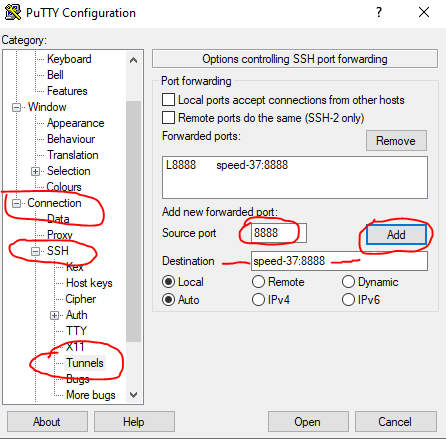
\includegraphics{images/putty1}}
	\caption{SSH tunnel configuration 1}
	\label{fig:putty1}
\end{figure}

\begin{figure}[htbp]
	\centering
	\fbox{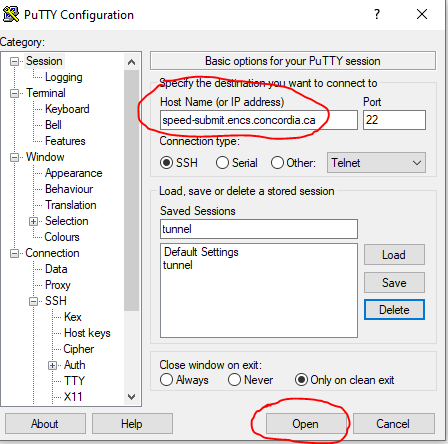
\includegraphics{images/putty2}}
	\caption{SSH tunnel configuration 2}
	\label{fig:putty2}
\end{figure}

\begin{figure}[htbp]
	\centering
	\fbox{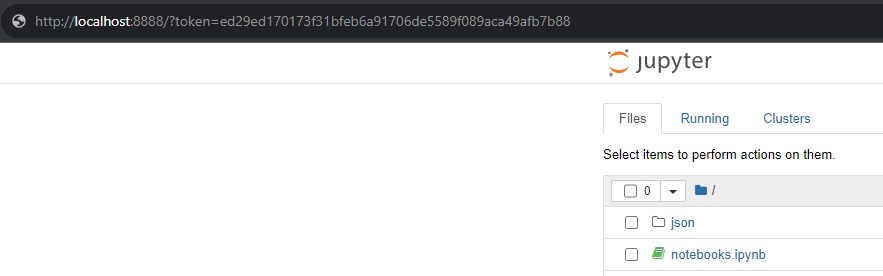
\includegraphics[width=0.9\textwidth]{images/jupyter.png}}
	\caption{Jupyter running on a Speed node}
	\label{fig:jupyter}
\end{figure}

\noindent Another sample is the OpenISS-derived containers with Conda and Jupyter,
see \xs{sect:openiss-examples} for details.

% 2.8.3.2 Jupyter Notebook in Conda
% ----------------------------------
\paragraph{Jupyter Notebook in Conda}
\label{sect:jupyter-conda}

For setting up Jupyter Labs with Conda and Pytorch, follow these steps:

\textbf{Environment preparation:} (only once, takes some time to run to install all required dependencies)
\begin{enumerate}
\item Start an interactive session, and navigate to your \tool{speed-scratch} directory:
\begin{verbatim}
salloc --mem=20G --gpus=1
cd /speed-scratch/$USER
\end{verbatim}

\item Load and initilize the environment
\begin{verbatim}
module load anaconda/2023.03/default
conda init tcsh
source ~/.tcshrc
\end{verbatim}

\item Set up Conda environment by runnung \tool{setup-conda.sh}
(on the compute node salloc brought you to, not on speed-submit)
as shown in \xf{fig:setup_conda.sh}
\begin{verbatim} ./setup_conda.sh \end{verbatim}

\small
\begin{figure}[htpb]
    \lstinputlisting[language=csh,frame=single,basicstyle=\ttfamily\scriptsize]{../../src/jupyter/jupyterlabs-conda/setup_conda.sh}
    \caption{Source code for \file{setup_conda.sh}}
    \label{fig:setup_conda.sh}
\end{figure}
\normalsize
\end{enumerate}

The script will:
\begin{itemize}
    \item create a Jupyter directory change Jupyter to any name of your choice in the script
    \item set environment variables
    \item create a conda environment named jupyter-env
    \item install JupyterLabs and pytorch
    \item exit the interactive session
\end{itemize}

\textbf{Launching Jupyter Labs instance from \textbf{speed-submit}:}
\begin{enumerate}
    \item Run the \tool{start\_jupyterlab.sh} script each time you need to launch JupyterLab from the submit node
    The script will:
    \begin{itemize}
        \item allocate resources for your job on a compute node
        \item start jupyter server by running \tool{run\_jupyterlab.sh}
        \item print the ssh command that you can use to connect to the compute node runnung the jupyter notebook (this is done in a new terminal)
        \item print the token/link to the jupyter server to paste in a web browser (starting with http://127.0.0.1/...)
    \end{itemize}

    \item Open a browser, and copy your Jupyter's token and paste it in the browser's URL field.
\end{enumerate}


% 2.8.3.3 Jupyter Notebook in Python Virtual Env
% ----------------------------------------------
\paragraph{Jupyter Notebook in Python venv}
\label{sect:jupyter-python}

This is an example of Jupyter Labs running in a Python Virtual environment on Speed.

\textbf{Note:} Use of Python virtual environments is preferred over Conda at Alliance Canada clusters.
If you prefer to make jobs that are more compatible between Speed and Alliance clusters, use Python
\texttt{venv}s. See \url{https://docs.alliancecan.ca/wiki/Anaconda/en}
and \url{https://docs.alliancecan.ca/wiki/JupyterNotebook}.

\begin{itemize}
\item Environment preparation: for the FIRST time only:
\begin{enumerate}
\item Go to your speed-scratch directory: \texttt{cd /speed-scratch/\$USER}
\item Open an interactive session: \texttt{salloc --mem=50G --gpus=1 --constraint=el9}
\item Create a Python \texttt{venv} and install \tool{jupyterlab}+\tool{pytorch}
\small
\begin{verbatim}
module load python/3.11.5/default
setenv TMPDIR /speed-scratch/$USER/tmp
setenv TMP /speed-scratch/$USER/tmp
setenv PIP_CACHE_DIR /speed-scratch/$USER/tmp/cache
python -m venv /speed-scratch/$USER/tmp/jupyter-venv
source /speed-scratch/$USER/tmp/jupyter-venv/bin/activate.csh
pip install jupyterlab
pip3 install torch torchvision torchaudio --index-url https://download.pytorch.org/whl/cu118
exit
\end{verbatim}
\normalsize
\end{enumerate}

\item Running Jupyter, from \textbf{speed-submit}:
\begin{enumerate}
\item Open an interactive session: \texttt{salloc --mem=50G --gpus=1 --constraint=el9}
\small
\begin{verbatim}
cd /speed-scratch/$USER
module load python/3.11.5/default
setenv PIP_CACHE_DIR /speed-scratch/$USER/tmp/cache
source /speed-scratch/$USER/tmp/jupyter-venv/bin/activate.csh
jupyter lab --no-browser --notebook-dir=$PWD --ip="0.0.0.0" --port=8888 --port-retries=50
\end{verbatim}
\normalsize

\item Verify which port the system has assigned to Jupyter: \texttt{http://localhost:XXXX/lab?token=}

\item SSH Tunnel creation: similar to Jupyter in Singularity, see \xs{sect:jupyter-singularity}

\item Open a browser and type: \texttt {localhost:XXXX} (using the port assigned)
\end{enumerate}
\end{itemize}


% 2.8.4 Visual Studio Code
% ------------------------
\subsubsection{Visual Studio Code}
\label{sect:vscode}

This is an example of running VS Code on Speed

\textbf{Note: } There are two ways to run Visual Studio Code (VS Code) on Speed.

% 2.8.4.1 Web-based Version
% ----------------------------------------------
\paragraph{Web-based Version}
\label{sect:web-based-vscode}
Similar to Jupyter notebooks.

\begin{enumerate}
    \item Start an interactive session: \texttt{salloc --job-name=vs-code --mem=10G}
    \item Run the script \texttt{./vscode\_web.sh} located in \tool{/src/vscode} directory. The script will:
    \begin{itemize}
        \item Create a vscode directory (with subdirectories run-user and workspace)
        \item Set the environment variable \texttt{XDG\_RUNTIME\_DIR} appropriately.
        \item Print the SSH tunnel command required to forward port 8080 from the compute node to your local machine.
        \item Launch code-server in the background, which generates a configuration file (including the VS Code password).
    \end{itemize}
    \item Connect from your local machine by performing the following steps:
    \begin{itemize}
        \item Open a new terminal window and run the SSH tunnel command printed by the script.
        \item Open your web browser and navigate to http://localhost:8080.
        \item If prompted for a password, use the password printed by the script.
    \end{itemize}
\end{enumerate}

\small
\begin{figure}[htpb]
    \lstinputlisting[language=csh,frame=single,basicstyle=\ttfamily\scriptsize]{../../src/vscode/vscode_web.sh}
    \caption{Source code for \file{vscode_web.sh}}
    \label{fig:vscode_web.sh}
\end{figure}
\normalsize

\begin{figure}[htbp]
	\centering
	\fbox{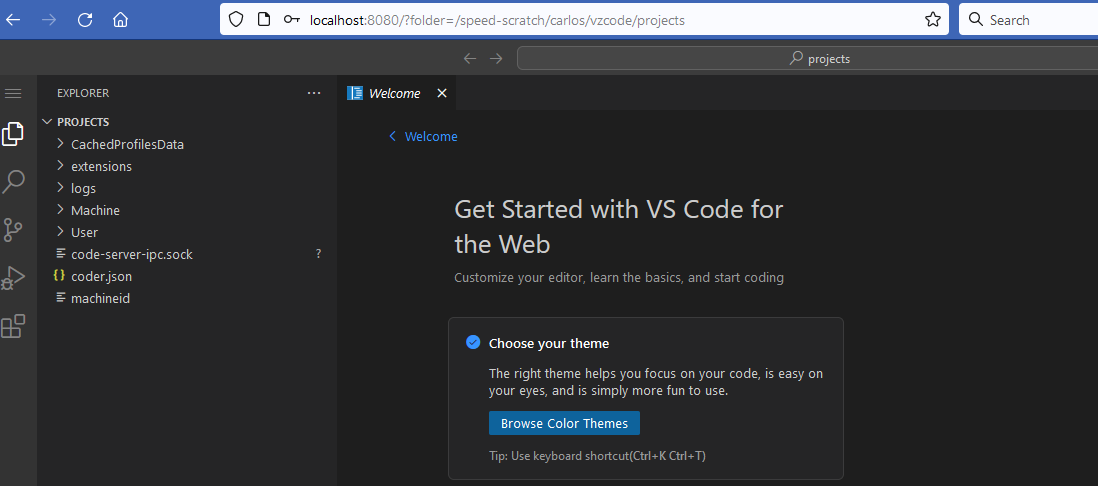
\includegraphics[width=0.9\textwidth]{images/vscode.png}}
	\caption{running VS Code (web) on a Speed node}
	\label{fig:vscode}
\end{figure}

% 2.8.4.2 Local Version
% ----------------------------------------------
\paragraph{Local Version}
\label{sect:local-vscode}
If you prefer to run VS Code directly on your local machine without relying on a browser-based code-server, 
detailed instructions are available in the \tool{/src/vscode} \href{https://github.com/NAG-DevOps/speed-hpc/blob/master/src/vscode}{README.md} file.